\subsection{Subsystem View}
The View subsystem encapsulates the parts of the system which control the GUI which the user sees. The ScoreView, VerboseView, and GameScene all display different parts of the state of the game Model, by binding themselves to Subject classes in the Model, in accordance with the Observer pattern. The ScoreView displays game state information. The VerboseView optionally shows logs of what is going on inside the Model. The GameScene is made up of 25 CardPanes which each observe Card objects in the model, changing the display when the Cards change state. By following the Observer pattern, the Model is allowed to exist without any View. The View provides a GUI, without effecting the Model subsystems.

\subsubsection{Detailed Design Diagram}

\begin{figure}[H]
\centering
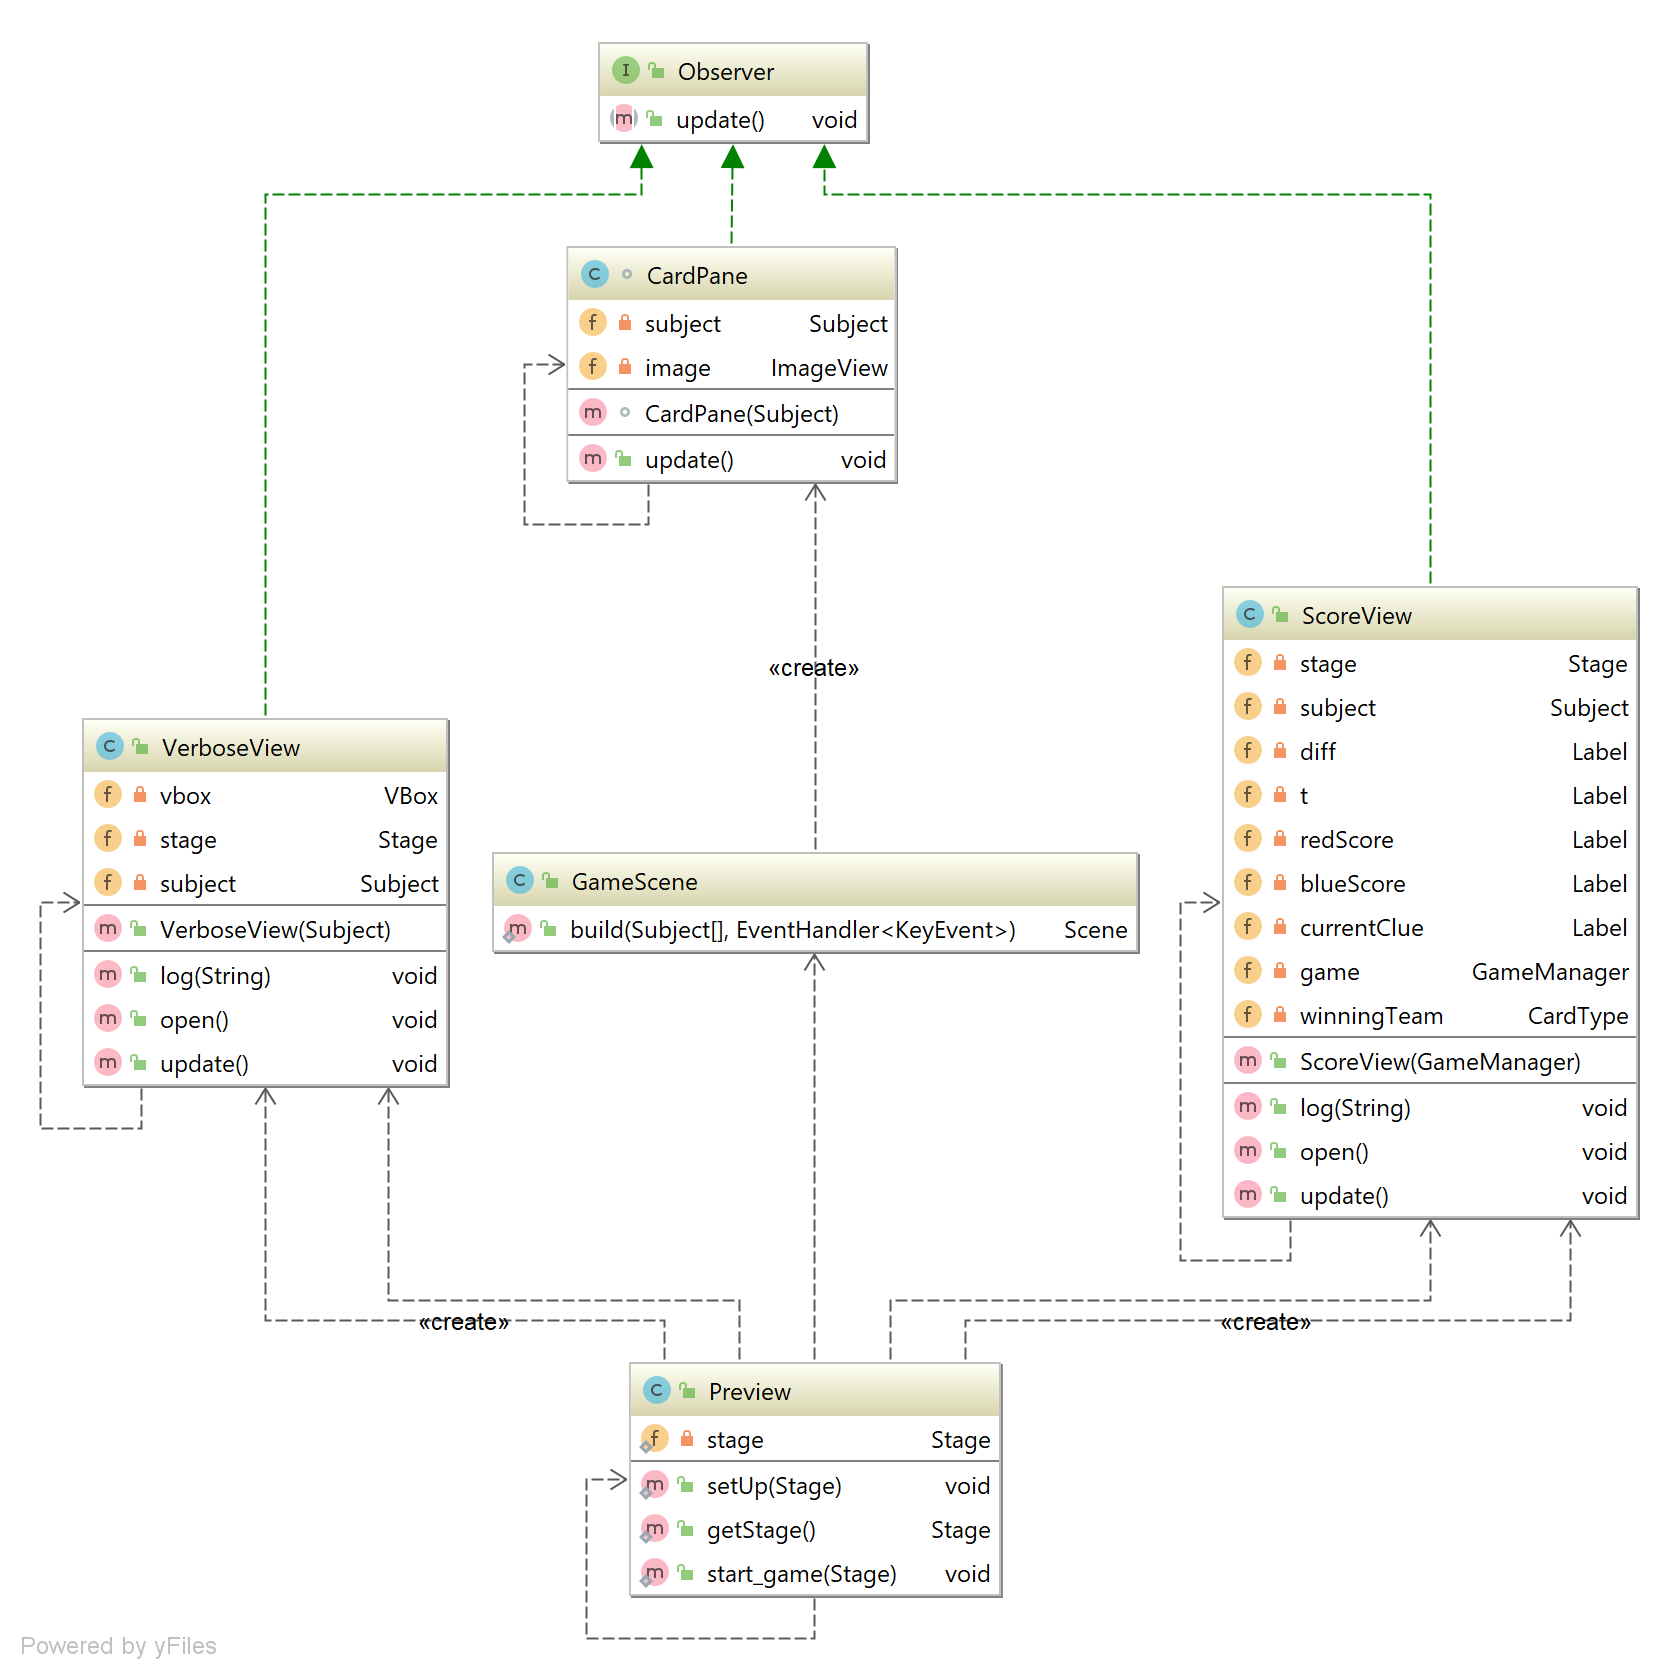
\includegraphics[width=10cm]{Source/Module/View/View.png}
\caption{UML Diagram of Module View}
\label{View}
\end{figure}

\subsubsection{Class Observer}
\begin{tabularx}{\textwidth}{|c||l|l|l|X|}
    \hline
    \cellcolor{lightgray}Class Name & \multicolumn{4}{X|}{Observer}\\
    \hline
    \cellcolor{lightgray}Inherits From & \multicolumn{4}{X|}{None}\\
    \hline
    \cellcolor{lightgray}Description & \multicolumn{4}{p{12cm}|}{Part of the Observer design pattern. Interface used for communication to the Subject.}\\
    \hline\hline
    
    \cellcolor{lightgray}Methods & \cellcolor{lightgray}Visibility & \multicolumn{2}{l|}{\cellcolor{lightgray}Method Name} & \cellcolor{lightgray}Description\\\cline{2-5}
    \cellcolor{lightgray} & Public & \multicolumn{2}{l|}{update()} & Update the state of the observer\\
    \hline
\end{tabularx}
\subsubsection{Class VerboseView}
\begin{tabularx}{\textwidth}{|c||l|l|l|X|}
    \hline
    \cellcolor{lightgray}Class Name & \multicolumn{4}{X|}{VerboseView}\\
    \hline
    \cellcolor{lightgray}Inherits From & \multicolumn{4}{X|}{Observer}\\
    \hline
    \cellcolor{lightgray}Description & \multicolumn{4}{p{12cm}|}{Maintains graphical representation of the game play during each turn phase}\\
    \hline\hline
    
    \cellcolor{lightgray}Attributes & \cellcolor{lightgray}Visibility & \cellcolor{lightgray}Data type & \cellcolor{lightgray}Name & \cellcolor{lightgray}Description\\\cline{2-5}
    \cellcolor{lightgray} & Private & VBox & vbox & Object container responsible for containing the information to display\\\cline{2-5}
    \cellcolor{lightgray} & Private & Stage & stage & Container supporting the vbox object during display \\\cline{2-5}
    \cellcolor{lightgray} & Private & Subject & subject & The subject to bind to\\
    \hline\hline
    
    \cellcolor{lightgray}Methods & \cellcolor{lightgray}Visibility & \multicolumn{2}{l|}{\cellcolor{lightgray}Method Name} & \cellcolor{lightgray}Description\\\cline{2-5}
    \cellcolor{lightgray} & Public & \multicolumn{2}{l|}{VerboseView(Subject s)} & Constructor that binds to the subject\\\cline{2-5}
    \cellcolor{lightgray} & Public & \multicolumn{2}{l|}{log(String arg)} & Updates the text information to display with specified arg statement\\\cline{2-5}
    \cellcolor{lightgray} & Public & \multicolumn{2}{l|}{open()} & Displays the score window\\\cline{2-5}
    \cellcolor{lightgray} & Public & \multicolumn{2}{l|}{update()} & Calls log method and passes subject message to it\\
    \hline
\end{tabularx}
\subsubsection{Class CardPane}
\begin{tabularx}{\textwidth}{|c||l|l|l|X|}
    \hline
    \cellcolor{lightgray}Class Name & \multicolumn{4}{X|}{CardPane}\\
    \hline
    \cellcolor{lightgray}Inherits From & \multicolumn{4}{X|}{StackPane, Observer}\\
    \hline
    \cellcolor{lightgray}Description & \multicolumn{4}{p{12cm}|}{Maintains graphical representation of a card during each game phase}\\
    \hline\hline
    
    \cellcolor{lightgray}Attributes & \cellcolor{lightgray}Visibility & \cellcolor{lightgray}Data type & \cellcolor{lightgray}Name & \cellcolor{lightgray}Description\\\cline{2-5}
    \cellcolor{lightgray} & Private & ImageView & image & Object responsible for loading character image files \\\cline{2-5}
    \cellcolor{lightgray} & Private & Subject & subject & The subject to bind to\\
    \hline\hline
    
    \cellcolor{lightgray}Methods & \cellcolor{lightgray}Visibility & \multicolumn{2}{l|}{\cellcolor{lightgray}Method Name} & \cellcolor{lightgray}Description\\\cline{2-5}
    \cellcolor{lightgray} & Protected & \multicolumn{2}{l|}{CardPane(Subject subject)} & Constructor that binds to the subject\\\cline{2-5}
    \cellcolor{lightgray} & Public & \multicolumn{2}{l|}{update()} & Updates the ImageView object to display the associated character image file\\
    \hline
\end{tabularx}


\subsubsection{Class GameScene}
\begin{tabularx}{\textwidth}{|c||l|l|l|X|}
    \hline
    \cellcolor{lightgray}Class Name & \multicolumn{4}{X|}{GameScene}\\
    \hline
    \cellcolor{lightgray}Inherits From & \multicolumn{4}{X|}{None}\\
    \hline
    \cellcolor{lightgray}Description & \multicolumn{4}{p{12cm}|}{Container for all CardPane objects. Factory for building graphical tree of all cards.}\\
    \hline\hline
    
    \cellcolor{lightgray}Methods & \cellcolor{lightgray}Visibility & \multicolumn{2}{l|}{\cellcolor{lightgray}Method Name} & \cellcolor{lightgray}Description\\\cline{2-5}
    \cellcolor{lightgray} & Public & \multicolumn{2}{X|}{build(Subject[] subjects, EventHandler\textlangle{}KeyEvent\textrangle{} handler)} & Constructs the game scene containing all card nodes, and returns it to the invoker\\
    \hline
\end{tabularx}
\subsubsection{Class ScoreView}
\begin{tabularx}{\textwidth}{|c||l|l|l|X|}
    \hline
    \cellcolor{lightgray}Class Name & \multicolumn{4}{X|}{ScoreView}\\
    \hline
    \cellcolor{lightgray}Inherits From & \multicolumn{4}{X|}{Observer}\\
    \hline
    \cellcolor{lightgray}Description & \multicolumn{4}{p{12cm}|}{Maintains a graphical representation of the score during the game play}\\
    \hline\hline
    
    \cellcolor{lightgray}Attributes & \cellcolor{lightgray}Visibility & \cellcolor{lightgray}Data type & \cellcolor{lightgray}Name & \cellcolor{lightgray}Description\\\cline{2-5}
    \cellcolor{lightgray} & Private & Stage & stage & Object container responsible for containing the attributes to display\\\cline{2-5}
    \cellcolor{lightgray} & Private & Subject & subject & The subject to bind to\\\cline{2-5}
    \cellcolor{lightgray} & Private & Label & diff & Object representing the difficulty\\\cline{2-5}
    \cellcolor{lightgray} & Private & Label & t & Object representing the team's turn\\\cline{2-5}
    \cellcolor{lightgray} & Private & Label & redScore & Object representing red team's score\\\cline{2-5}
    \cellcolor{lightgray} & Private & Label & blueScore & Object representing blue team's score\\\cline{2-5}
    \cellcolor{lightgray} & Private & Label & currentClue & Object representing the current clue of the turn\\\cline{2-5}
    \cellcolor{lightgray} & Private & GameManager & game & Reference of the current game object to receive notifications from\\\cline{2-5}
    \cellcolor{lightgray} & Private & CardType & winningTeam & Team currently in the lead\\
    \hline\hline
    
    \cellcolor{lightgray}Methods & \cellcolor{lightgray}Visibility & \multicolumn{2}{l|}{\cellcolor{lightgray}Method Name} & \cellcolor{lightgray}Description\\\cline{2-5}
    \cellcolor{lightgray} & Public & \multicolumn{2}{l|}{ScoreView(GameManager game)} & Constructor\\\cline{2-5}
    \cellcolor{lightgray} & Public & \multicolumn{2}{l|}{log(String arg)} & Updates the labels to reflect the current state of the game\\\cline{2-5}
    \cellcolor{lightgray} & Public & \multicolumn{2}{l|}{open()} & Displays the score window\\\cline{2-5}
    \cellcolor{lightgray} & Public & \multicolumn{2}{l|}{update()} & Calls log method and passes subject message to it\\
    \hline
\end{tabularx}

